\documentclass{article}

\usepackage{graphicx}
\usepackage[left=2.5cm, right=2.5cm, top=2cm, bottom=2cm]{geometry}
\usepackage{titlesec}
\usepackage{amsmath}
\usepackage{algorithm}
\usepackage{algpseudocode}
\usepackage{tikz}
\usepackage{caption}
\usepackage{listings}
\usepackage{xcolor}
\usepackage{fancyhdr}
\usepackage{changepage}
\usepackage{svg}
\usepackage{float} % 提供更灵活的图片位置控制
\pagestyle{fancy}
\fancyhf{} % 清空页眉和页脚
\fancyfoot[C]{\thepage} % 只在页脚中居中显示页码
\renewcommand{\headrulewidth}{0pt} % 去掉页眉的横线
\usetikzlibrary{trees, shapes.geometric, arrows, positioning}
\usepackage{lmodern}
\usepackage[UTF8]{ctex}
\usepackage{xeCJK}
    \setCJKmainfont[AutoFakeBold=3]{TW-Sung}
    \XeTeXlinebreaklocale "zh"
    \XeTeXlinebreakskip = 0pt plus 1pt
\usepackage{multirow}
\ctexset{
    figurename = {Figure},
    tablename = {Table}
}



% ER Diagram的參數
% 定義字體樣式和透明度
\tikzstyle{entity} = [rectangle, minimum width=3cm, minimum height=1cm, text centered, draw=black, fill=lightgray, fill opacity=0.7, font=\ttfamily]
\tikzstyle{attribute} = [ellipse, minimum width=2cm, minimum height=1cm, text centered, draw=black, fill=lightblue, fill opacity=0.7, font=\ttfamily]
\tikzstyle{relationship} = [diamond, minimum width=2cm, minimum height=1cm, text centered, draw=black, fill=lightgray, fill opacity=0.7, font=\ttfamily]
\tikzstyle{arrow} = [thick,->,>=stealth, draw opacity=0.7]

\titleformat{\section}[hang]{\normalfont\Large\bfseries}{\thesection}{1em}{}
\titleformat{\subsection}[hang]{\normalfont\bfseries}{\thesubsection}{2em}{}
\titleformat{\subsubsection}[hang]{\normalfont\bfseries}{\thesubsubsection}{5em}{}

\titlespacing*{\subsection}{2em}{3.25ex plus 1ex minus .2ex}{1.5ex plus .2ex}
\titlespacing*{\subsubsection}{3em}{3.25ex plus 1ex minus .2ex}{1.5ex plus .2ex}

\lstset{
    language=SQL,
    basicstyle=\ttfamily\small,
    keywordstyle=\color{blue},
    commentstyle=\color{brown},
    stringstyle=\color{red},
    showstringspaces=false,
    numbers=left,
    numberstyle=\tiny\color{gray},
    stepnumber=1,
    numbersep=5pt,
    backgroundcolor=\color{white},
    frame=single,
    rulecolor=\color{black},
    captionpos=b,
    inputencoding=utf8,
    extendedchars=true
}


\title{Database Management\\Homework 2}
\author{B11705044 \\ Yen-Hung, Chiang}
\date{}

\begin{document}

\maketitle

\section*{1}
\subsection*{(a)}
\subsubsection*{(i)}
\begin{adjustwidth}{3em}{}
是,\texttt{INSTRUCTOR} 連到 \texttt{DEAN} 的線上標示 (0,1),代表一個教師最多只可以當一個學院的院長。
\end{adjustwidth}

\subsubsection*{(ii)}
\begin{adjustwidth}{3em}{}
否,\texttt{INSTRUCTOR} 連到 \texttt{TEACHES} 的地方標示 (0,N),代表一個教師可以不教課也可以教多個班次的課。\texttt{SECTION} 連到 \texttt{TEACHES} 的地方標示 (1,1),代表一個班次的課必須由恰好一個教師負責。
\end{adjustwidth}

\subsubsection*{(iii)}
\begin{adjustwidth}{3em}{}
否,\texttt{STUDENT} 連到 \texttt{HAS} 的線上標示 (0,1),代表一個學生最多可以隸屬一個系,也可以不隸屬任何系。\texttt{DEPT} 連到 \texttt{HAS} 的線上標示 (0,N),代表每
個學系可以擁有零位、一位或多位學生。
\end{adjustwidth}

\subsubsection*{(iv)}
\begin{adjustwidth}{3em}{}
是,\texttt{STUDENT} 連到 \texttt{TAKES} 這個動作的時候有標示 (0,N),代表學生可以修零個、一個或多個班次。\texttt{TAKES} 連到 \texttt{SECTION} 的線上標示 (5,N),代表一個班次至少要有五名學生修課。
\end{adjustwidth}

\subsubsection*{(v)}
\begin{adjustwidth}{3em}{}
是,因為 \texttt{CoName} 是 key attribute,所以不能重複。
\end{adjustwidth}

\subsection*{(b)}
下圖 (Figure 1)為根據題目要求繪製出的 relational schema diagram。
\begin{figure}[H] % 使用 figure 环境自动生成图片编号
    \centering
    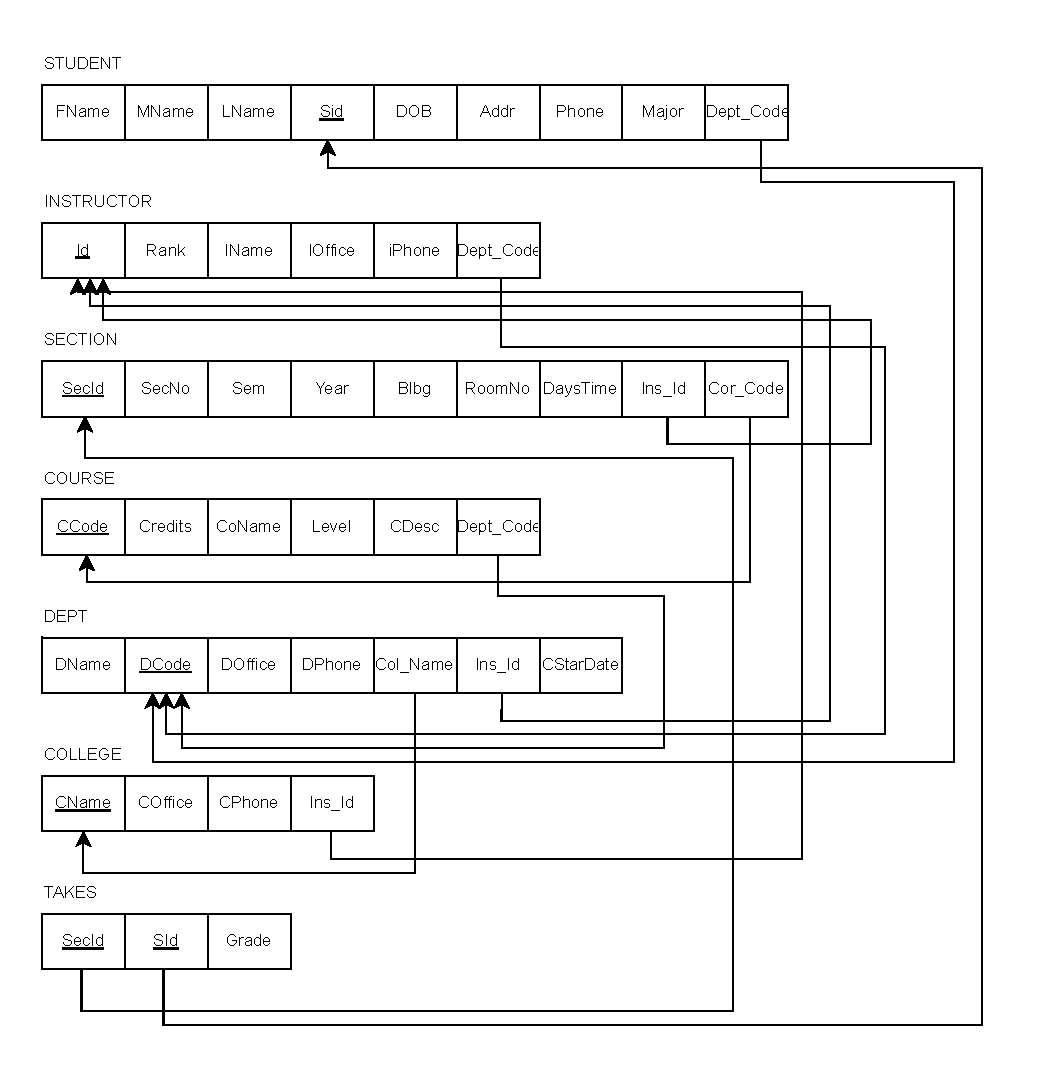
\includegraphics[scale=0.8]{1_b.pdf} % 插入图片
    \caption{Relational schema diagram} % 自动生成编号并添加标题
\end{figure}
\subsection*{(c)}
\begin{adjustwidth}{3em}{}
這個資料庫裡應該會有七張表,其中有六張表分別對應著 \texttt{STUDENT}、\texttt{INSTRUCTOR}、\texttt{DEPT}、\texttt{SECTION}、\texttt{COLLEGE}、\texttt{COURSE} 六個 entity,另外一張表 \texttt{TAKES} 紀錄了 \texttt{STUDENT} 和 \texttt{SECTION} 的關係。以下是各個 entity 之間的關係。
\begin{itemize}
\item 每個課程可以分成好幾個不同的班次也可以不分,且每個班次都一定要屬於一門課。
\item 一個學系可以提供好幾個課程也可以不提供,每門課只能屬於一個學系。
\item 一個學院可以有很多個學系也可以沒有,每個學系都只屬於一個學院。
\item 每個學院一定且只能有一位教師當院長,一位教師最多只能當一個學院的院長也可以不當。
\item 每個學系一定且只能有一位教師當系主任,一位教師最多只能當一個學系的系主任也可以不當。
\item 每個教師一定且只能被一個學系雇用,每個學系可以雇用多位教師也可以不雇用。
\item 每個班次的課一定且只能被一位教師教,一位教師可以上很多班次的課也可以不上。
\item 每個系可以有很多位學生也可以沒有任何學生,而每位學生最多可以屬於一個系也可以不屬於任何系。
\item 最後每位學生可以選多個班次的課也可以不選,但每個班次的課至少要有五個以上的學生才成立,而 \texttt{TAKES} 就是在記錄這個關係。
\end{itemize}



\end{adjustwidth}

\section*{2}
\subsection*{(a)}
下圖(Figure 2)為根據題目要求繪製出的實體關聯圖。圖中共有四個實體,分別為 \texttt{STUDENT}、\texttt{APPLICATION}、\texttt{LOCKER}、以及\texttt{SEMESTER}。
\begin{itemize}
\item \texttt{STUDENT} 記載了學生的學號 (\texttt{Student\_Id})。
\item \texttt{APPLICATION} 記載了申請編號(\texttt{Application\_Id})、請求幾個大櫃子(\texttt{Large\_Cnt})、幾個小櫃子(\texttt{Small\_Cnt})、以及是否取消(\texttt{Is\_Canceled})。
\item \texttt{SEMESTER} 記載了學期編號(\texttt{Semester\_Id})、以及每學期可用的系櫃數量(\texttt{Available\_Lockers})。 
\item \texttt{LOCKER} 記載了系櫃編號(\texttt{Locker\_Id})、系櫃尺寸(\texttt{Size})、以及處於何種狀態(\texttt{Status})。
\end{itemize}
\begin{figure}[H] % 使用 figure 环境自动生成图片编号
    \centering
    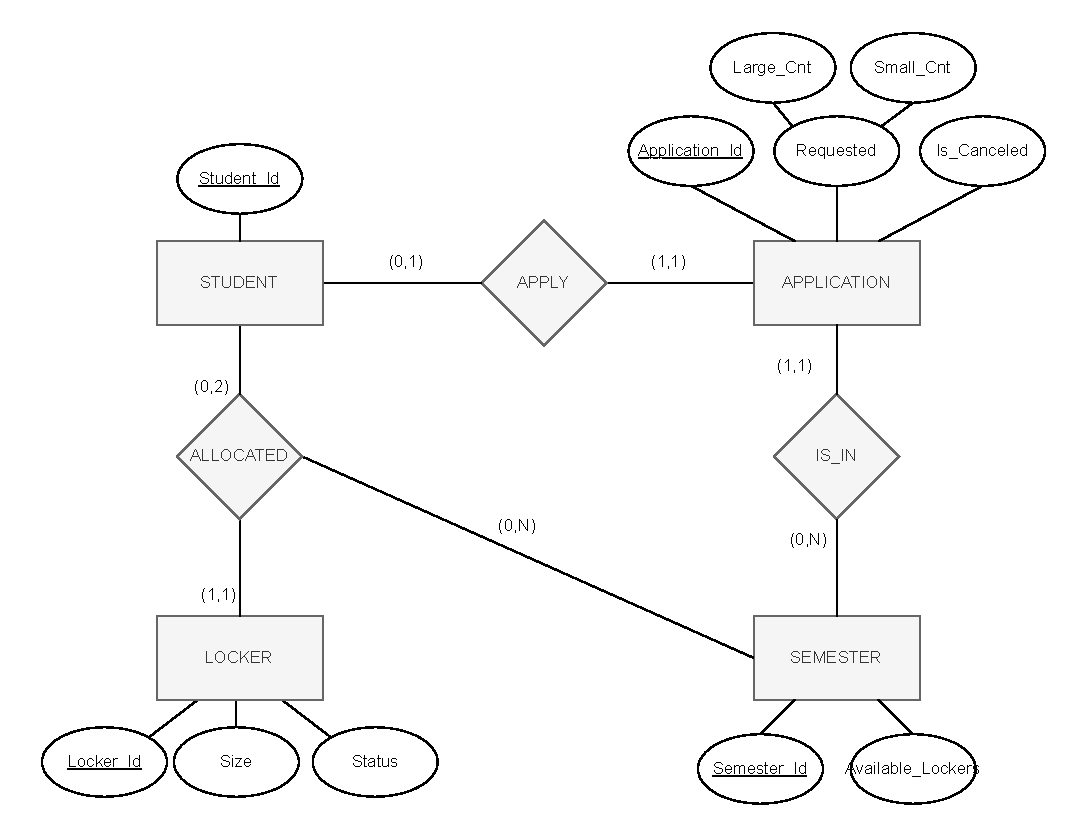
\includegraphics[scale=0.7]{2_a_4.pdf} % 插入图片
    \caption{ER-diagram} % 自动生成编号并添加标题
\end{figure}

\subsection*{(b)}
下圖(Figure 3)為根據 (a) 小題繪製出來的 relational schema diagram。
\begin{figure}[H] % 使用 figure 环境自动生成图片编号
    \centering
    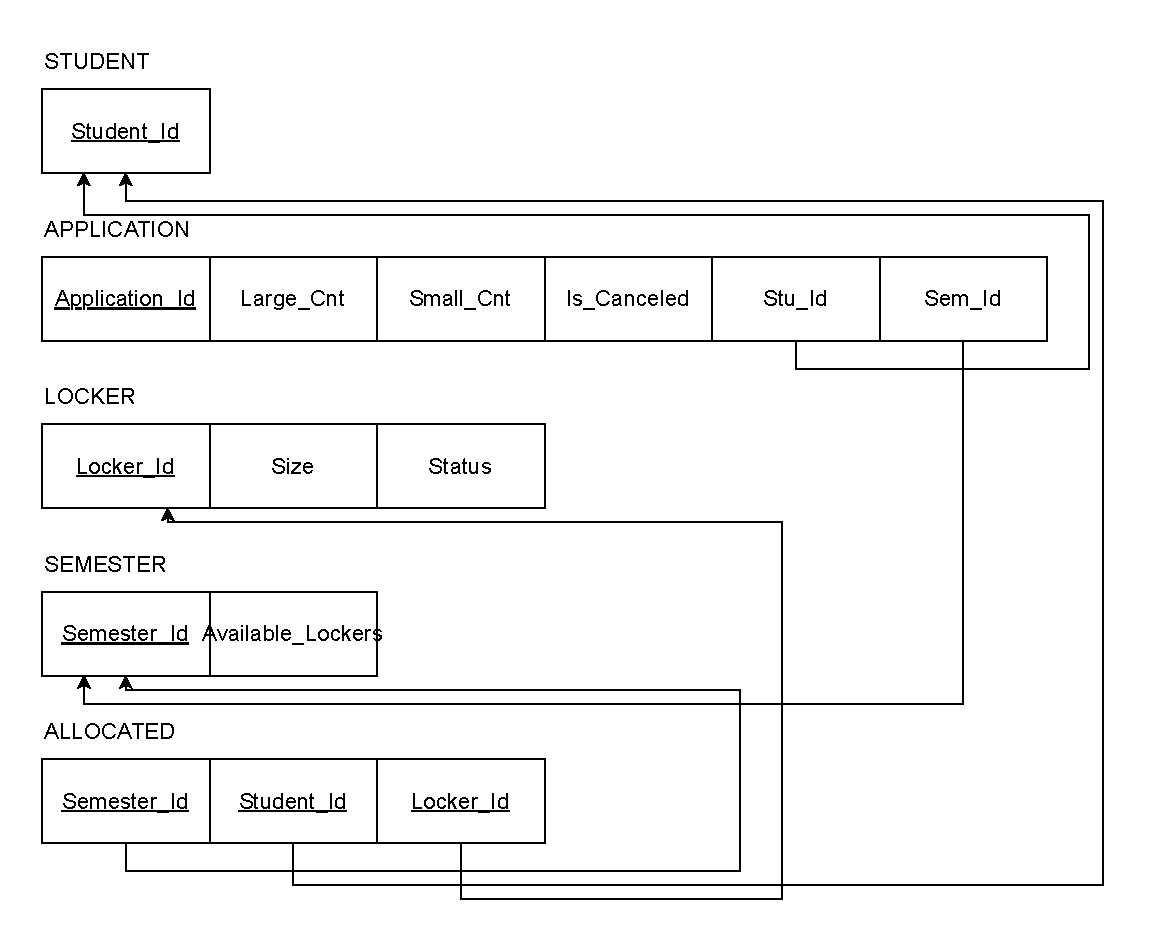
\includegraphics[scale=0.6]{2_b_3.pdf} % 插入图片
    \caption{Relational schema diagram} % 自动生成编号并添加标题
\end{figure}

\subsection*{(c)}
下面的 SQL 程式碼(Listing 1)會在資料庫中產生 (b) 小題的 schema。
\begin{lstlisting}[caption={SQL schema for the locker rental system}]
CREATE TABLE STUDENT(
	Student_Id INT NOT NULL,
	PRIMARY KEY(Student_Id)
);

CREATE TABLE SEMESTER(
	Semeter_Id INT NOT NULL,
	Available_Locker INT NOT NULL,
	PRIMARY KEY(Semeter_Id)
);

CREATE TABLE APPLICATION(
	Application_Id INT NOT NULL,
	Large_Cnt INT,
	Small_Cnt INT,
	Is_Canceled VARCHAR(10) NOT NULL,
	Stu_Id INT NOT NULL,
	Sem_Id INT NOT NULL,
	PRIMARY KEY(Application_Id),
	FOREIGN KEY(Stu_Id) REFERENCES STUDENT(Student_Id),
	FOREIGN KEY(Sem_Id) REFERENCES SEMESTER(Semeter_Id)
);

CREATE TABLE LOCKER(
	Locker_Id INT NOT NULL,
	Size_ CHAR NOT NULL,
	Status VARCHAR(20) NOT NULL,
	PRIMARY KEY(Locker_Id)
);

CREATE TABLE ALLOCATED(
	Semeter_Id INT NOT NULL,
	Student_Id INT NOT NULL,
	Locker_Id INT NOT NULL,
	PRIMARY KEY(Semeter_Id, Student_Id, Locker_Id),
	FOREIGN KEY(Semeter_Id) REFERENCES SEMESTER(Semeter_Id),
	FOREIGN KEY(Student_Id) REFERENCES STUDENT(Student_Id),
	FOREIGN KEY(Locker_Id) REFERENCES LOCKER(Locker_Id)
);
\end{lstlisting}

\section*{3}
\subsection*{(a)}
下面一句 SQL 指令(Listing 2)可以給定一個指定的學期後,列出所有被分配到兩格的學生,以及所有有申請但沒有被分配到的學生。
\begin{lstlisting}[caption={SQL for 分配原則}]
WITH StudentAllocations AS (
    SELECT 
        A.Stu_Id AS Student_Id, 
        SUM(A.Large_Cnt + A.Small_Cnt) AS Total_Applications, 
        COUNT(AL.Locker_Id) AS Total_Allocated
    FROM 
        APPLICATION A
    LEFT JOIN 
        ALLOCATED AL ON A.Stu_Id = AL.Student_Id AND A.Sem_Id = AL.Semeter_Id
    WHERE 
        A.Sem_Id = ? -- 指定學期
    GROUP BY 
        A.Stu_Id
)
SELECT 
    Student_Id, 
    Total_Applications, 
    Total_Allocated
FROM 
    StudentAllocations
WHERE 
    Total_Allocated = 2

UNION ALL

SELECT 
    Student_Id, 
    Total_Applications, 
    Total_Allocated
FROM 
    StudentAllocations
WHERE 
    Total_Allocated = 0
ORDER BY 
    Total_Allocated DESC;

\end{lstlisting}


\subsection*{(b)}
\begin{lstlisting}[caption={第一句 SQL}]
SELECT 
    A1.Stu_Id AS Student_Id
FROM 
    APPLICATION A1
LEFT JOIN 
    ALLOCATED AL1 ON A1.Stu_Id = AL1.Student_Id AND A1.Sem_Id = AL1.Sem_Id
WHERE 
    A1.Sem_Id = ?  -- 指定學期
    AND A1.Sem_Id = A1.Sem_Id - 1  -- 前一學期
    AND AL1.Locker_Id IS NULL  

UNION ALL

SELECT 
    A2.Stu_Id AS Student_Id
FROM 
    APPLICATION A2
LEFT JOIN 
    ALLOCATED AL2 ON A2.Stu_Id = AL2.Student_Id AND A2.Sem_Id = AL2.Sem_Id
WHERE 
    A2.Sem_Id = ?  -- 指定學期
    AND AL2.Locker_Id IS NULL  

UNION ALL

SELECT 
    A3.Stu_Id AS Student_Id
FROM 
    APPLICATION A3
JOIN 
    ALLOCATED AL3 ON A3.Stu_Id = AL3.Student_Id AND A3.Sem_Id = AL3.Sem_Id
WHERE 
    A3.Sem_Id = ?  -- 指定學期
    AND AL3.Locker_Id IS NOT NULL 
    AND A3.Sem_Id = A3.Sem_Id - 1;  

\end{lstlisting}

\begin{lstlisting}[caption={第二句 SQL}]
SELECT 
    A4.Stu_Id AS Student_Id
FROM 
    APPLICATION A4
JOIN 
    ALLOCATED AL4 ON A4.Stu_Id = AL4.Student_Id AND A4.Sem_Id = AL4.Sem_Id
WHERE 
    A4.Sem_Id = ?  -- 指定學期
    AND AL4.Locker_Id IS NOT NULL  
    AND (SELECT COUNT(*) 
         FROM ALLOCATED AL 
         WHERE AL.Student_Id = A4.Stu_Id 
         AND AL.Semeter_Id = A4.Sem_Id - 1) = 1  -- 前一學期被分配到恰好一格

UNION ALL

SELECT 
    A5.Stu_Id AS Student_Id
FROM 
    APPLICATION A5
JOIN 
    ALLOCATED AL5 ON A5.Stu_Id = AL5.Student_Id AND A5.Sem_Id = AL5.Sem_Id
WHERE 
    A5.Sem_Id = ?  -- 指定學期
    AND AL5.Locker_Id IS NOT NULL
    AND (SELECT COUNT(*) 
         FROM ALLOCATED AL 
         WHERE AL.Student_Id = A5.Stu_Id 
         AND AL.Semeter_Id = A5.Sem_Id - 1) = 2;  -- 前一學期被分配到恰好兩格
\end{lstlisting}


\subsection*{(c)}
下面兩句 SQL 指令分別可以讓學生修改申請(Listing 5)、和取消申請(Listing 6)。
\begin{lstlisting}[caption={學生修改申請}]
UPDATE APPLICATION
SET Large_Cnt = ?, -- 申請數量 
    Small_Cnt = ? -- 申請數量 
WHERE Stu_Id = ? -- 學號 
  AND Sem_Id = ? -- 當學期的學期 Id 
  AND Is_Canceled = 'No';  

\end{lstlisting}

\begin{lstlisting}[caption={學生取消申請}]
UPDATE APPLICATION
SET Is_Canceled = 'Yes'
WHERE Stu_Id = ? -- 學號
  AND Sem_Id = ? -- 當學期的學期 Id
  AND Is_Canceled = 'No'; 
\end{lstlisting}

\end{document}
